\documentclass{ctexart}
\usepackage{amsmath}
\usepackage{graphicx}
\usepackage{esint}

\usepackage{geometry}
\geometry{left=3.18cm,right=3.18cm,top=2.54cm,bottom=2.54cm}

\bibliographystyle{unsrt}

\newtheorem{deff}{定义}

\newcommand{\epsz}{\epsilon_0}
\newcommand{\epsr}{\epsilon_r}
\newcommand{\bfr}{\mathbf r}
\newcommand{\epsrr}{\epsr(\bfr)}
\newcommand{\epszr}{\epsz\epsrr}
\newcommand{\dd}[2]{\frac{\mathrm d #1}{\mathrm d #2}}

\title{关于电介质液面上升问题的讨论}
\author{杨天骅}

\begin{document}
	\maketitle
	\tableofcontents
	
	\newpage
	
	\section{简介}
	
	本文试图讨论一道在物理竞赛界非常有名且争议不断的题目,原题陈述如下:
	
	{\itshape 水平放置的平行板电容器,一块极板在液面上方,另一块极板浸没在液面下,如图\ref{fig:orig}所示。液体的相对介电常数为$\epsr$,密度为$\rho$。传给电容器极板电荷面密度$\sigma$后,电容器中的液面升高多少?}
	
	\begin{figure}[htbp!]
		\centering
		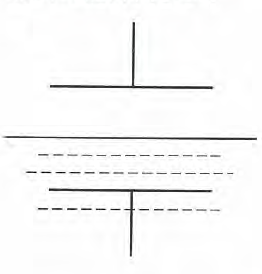
\includegraphics{Orig.png}
		\caption{原题图}
		\label{fig:orig}
	\end{figure}
	
	原书\footnote{\textit{舒幼生,第三章第一节}}中给出了一种基于受力的做法(以下称为“经典受力法”),而后同学们发现,如果用虚功原理处理此题,得到的结论将与经典受力法不同。此后围绕这两种做法、以及整个含电介质的静电学问题展开了诸多讨论。本文试图汇总这些讨论,并给出一个统一自洽的解释。
	
	本文中用到的很多数学工具和物理概念都是超物理竞赛的纲的,对于学习物理竞赛的同学主要了解其中的物理思想——特别是关于电介质的物理图像——即可,有兴趣看懂数学细节的同学可以阅读矢量分析相关书籍。本文中的讨论难免有疏忽,如果有问题欢迎联系\footnote{thomasyangth@qq.com}和讨论。
	
	\section{关于电介质概念的释疑}
	
	为了让讨论能够进行,首先我们要明确电介质的概念。现实中的电介质是非常复杂的。一般来说,我们考虑电介质时,都用的是这样的方程:
	\begin{equation}\label{ME1}
	\nabla\cdot\mathbf D=\rho
	\end{equation}
	\begin{equation}\label{ME2}
	\nabla\times\mathbf E=0
	\end{equation}
	\begin{equation}\label{ME3}
	\mathbf D(\mathbf r)=\epsilon_0\epsr(\mathbf r)\mathbf E(\mathbf r)
	\end{equation}
	\textit{对于不熟悉微分算符的读者,前两式等价于它们的积分形式:}
	\begin{equation}\label{ME1I}
	\oiint_{\partial V} \mathbf D\cdot \mathrm d\mathbf S=\iiint_V\rho \mathrm dV
	\end{equation}
	\begin{equation}\label{ME2I}
	\oint_l \mathbf E\cdot\mathrm d\mathbf r=0
	\end{equation}
	在这一道题目中,笔者认为应该采取这样一种电介质模型\footnote{为简化起见,只考虑静场情况。当然推广到含时情况和磁介质都是很自然的。}:
	
	{\itshape 电介质是一种分布在空间中的标量场$\epsr(\mathbf r)$,使得方程组\eqref{ME1},\eqref{ME2},\eqref{ME3}成立,其中$\rho$指自由电荷密度。}

	也就是说我们把上面几个方程当作了电介质的定义式。注意,这一定义中\textbf{完全不涉及“极化电荷”的概念},同样\textbf{不涉及电介质的任何微观结构}。它纯粹是一个宏观的理想模型,通俗一点说就是,我们不管它是不是鸭子,我们只要知道它长得像鸭子叫起来像鸭子就可以了。在这一定义下我们同样可以引入“极化强度”,此时$\mathbf P=\mathbf D-\epsz\mathbf E$成为它的定义式,从而它不再具有“单位体积内的电偶极矩”的意义,只是一个简化表达式的辅助量。
	
	这一定义主要排除了两种情况,一种是极化依赖于历史的、即有类似于磁滞的“电滞”现象的——我们这里假设电位移只和此刻的自由电荷分布有关;一种是电位移对电场的依赖不局域的,这种电介质的极化强度应该写为$\mathbf D(\mathbf r)=\iiint \chi(\mathbf r,\mathbf r^\prime)\mathbf E(\mathbf r^\prime)\mathrm d^3\mathbf r^\prime$,即一处的$\mathbf D$会依赖于其它处的$\mathbf E$。\footnote{这里的“依赖”指的是纯粹方程形式上的依赖,如果说物理上的话那么一处的电荷/电场变化确实会影响到另一处的电位移,但这可以是通过局域作用“传递”过去的。}
	
	现实中的电介质当然是有微观结构的,那么为了让我们下面算出来的结论有效,我们就要要求\textbf{通过这些微观结构给出来的电介质的宏观行为和我们上面定义的电介质的行为一致}。对于比较好的电介质这一假设是可以成立的\footnote{我猜可以吧……不然我们为什么要学这样的模型呢(逃},特别地,这种电介质可以用我们常用的在外电场作用下会产生一个正比于外电场的电偶极矩密度的系统来“实现”\footnote{只要假设这一点就足以推出上面的方程了,参见\textit{Jackson, Section 4.3}.}。从而下面我们讨论时务必分清两种情况:一种是只讨论抽象电介质的情况,此时有意义的只有自由电荷,用到的方程就是\eqref{ME1},\eqref{ME2},\eqref{ME3};如果要讨论到极化电荷等涉及电介质具体结构的内容,则进入考虑电介质微观结构的图景,此时可以用真空情况下的麦克斯韦方程。
	
	\section{电势能的概念}
	
	本题中另一个很让人困惑的概念就是电势能。电势能究竟应该如何计算?在本题的不同做法中,我们大致可以见到以下几种电势能的算法:
	\begin{equation}\label{W1}
	U=\sum_{\text{free}}\frac{1}{2}q_i\varphi_i=\frac{1}{2}\iiint \rho_f\varphi\mathrm dV
	\end{equation}
	\begin{equation}\label{W2}
	U=\sum_{\text{all}}\frac{1}{2}q_i\varphi_i=\frac{1}{2}\iiint \rho\varphi\mathrm dV
	\end{equation}
	\begin{equation}\label{W3}
	U=\iiint \frac{1}{2}\mathbf D\cdot\mathbf E\mathrm dV
	\end{equation}
	利用矢量分析,可以证明\eqref{W1}和\eqref{W3}是等价的:
	\begin{multline}
	\frac{1}{2}\iiint \rho_f\varphi\mathrm dV=\frac{1}{2}\iiint \varphi\nabla\cdot\mathbf D\mathrm dV\\=\frac{1}{2}\iiint \nabla\cdot(\varphi \mathbf D)-\mathbf D\cdot\nabla\varphi\mathrm dV=\underbrace{\frac{1}{2}\oiint \varphi\mathbf D\cdot\mathrm dS}_{=0}+\iiint\frac{1}{2}\mathbf D\cdot\mathbf E\mathrm dV
	\end{multline}
	其中面积分为零是因为我们在全空间积分,从而边界在无穷远处,如果无穷远处没有电荷的话,可以验证该边界积分在边界趋于无穷大时是趋于零的。
	
	这样我们知道\eqref{W2}和\eqref{W3}应该不等价。事实上:
	\begin{multline}
	\frac{1}{2}\iiint \rho\varphi\mathrm dV=\frac{1}{2}\iiint \epsilon_0\varphi\nabla\cdot\mathbf E\mathrm dV\\=\frac{\epsilon_0}{2}\iiint \nabla\cdot(\varphi \mathbf E)-\mathbf E\cdot\nabla\varphi\mathrm dV=\underbrace{\frac{\epsilon_0}{2}\oiint \varphi\mathbf E\cdot\mathrm dS}_{=0}+\iiint\frac{1}{2}\epsilon_0\mathbf E^2\mathrm dV
	\end{multline}
	
	也就是说,$\frac{1}{2}\rho_f\rho$和$\frac{1}{2}\mathbf D\cdot\mathbf E$对应,$\frac{1}{2}\rho\varphi$和$\frac{1}{2}\epsilon_0\mathbf E^2$对应,那么两者相减就应该得到$-\frac{1}{2}\rho_p\varphi$和$\frac{1}{2}\mathbf E\cdot\mathbf P$对应\footnote{这看起来很反直觉——$\rho\varphi$应该就是势能,为什么会带一个负号?我们下面会专门来讨论这一项的意义并回答这个问题}。
	
	这里必须明确一点的是,这个“对应”\textbf{是全局意义上的}。从上面的推导可以看出,我们只保证了\textbf{全空间的}$\frac{1}{2}\iiint \rho\varphi\mathrm dV$和$\iiint\frac{1}{2}\mathbf D\cdot\mathbf E\mathrm dV$相等。对于任意一个非全局的区域这个对应一般不成立。
	
	那么,接下来的问题是,我们应该用哪个?
	
	一般来说习惯竞赛或者普物电磁学思路的同学大概会觉得\eqref{W2}比较有道理。这是因为在竞赛的框架下,被认为是电势能“最基本”的表达式是:
	\begin{equation}\label{ClasU}
	U=\sum_{(i,j)}\frac{q_iq_j}{4\pi\epsilon_0 r_{ij}}
	\end{equation}
	按照这个思路来的话最自然得到的确实是\eqref{W2},因为看起来也没什么理由把极化电荷排斥在\eqref{ClasU}之外。
	
	但笔者认为这个做法是不对的。让我们回到“能量”最初的定义上面。牛顿力学的理论框架是基于力的,能量是一个派生概念,它定义为\textbf{一个系统能够对外做的功}。在这个定义下,\eqref{ClasU}是这么得来的:假设从系统现有的位型开始,我们一个一个地把这些电荷移动到无穷远,那么这个过程中静电力做的功就是\eqref{ClasU}。因此,对于“真空中的若干自由电荷”这样的模型,\eqref{ClasU}确实适用。
	
	但对于电介质情况,情况有所不同。如果此时继续使用\eqref{ClasU},得到的应该是\textbf{把包括极化电荷在内的所有电荷移动到无穷远做的功}。这就显得有些不对了:系统的“基态”并不是极化电荷彼此处于无穷远的状态。事实上,如果介质不能动的话,极化电荷的移动是不能做机械功的!\footnote{只要稍微想一下,我们能够通过两个自由电荷相互排斥来获得机械功,但我们如何能利用一个极化了的电介质里的电荷受到的力来做功呢?(暂时不考虑介质移动)}这样很自然地得出结论:如果介质不能动,那么系统的势能的微分应该等于自由电荷受到的静电力做的功。具体地,假设原先自由电荷分布为$\rho_f(\mathbf r)$,$\mathbf r$处的自由电荷有一位移$\xi(\mathbf r)$,则这一做功应该为\footnote{$\delta W$为正代表静电能增加}
	\begin{equation}
	W=-\iiint \rho_f(\mathbf r)\xi(\mathbf r)\cdot \mathbf E(\mathbf r)\mathrm dV
	\end{equation}
	利用$E=-\nabla\varphi$,上式化为
	\begin{equation}
	\iiint \rho_f(\mathbf r)\xi(\mathbf r)\cdot \nabla\varphi(\mathbf r)\mathrm dV=\oiint \rho_f(\mathbf r)\xi(\mathbf r)\varphi(\mathbf r)\cdot\mathrm d\mathbf S-\iiint \varphi(\mathbf r)\nabla\cdot\left(\rho_f(\mathbf r)\xi(\mathbf r)\right)\mathrm dV
	\end{equation}
	假设无穷远处无电荷(或电荷密度足够快地趋于零),则边界项消失。再利用\footnote{这里$\delta\rho_f$指所有自由电荷位移$\xi$后新的电荷密度相对于原来自由电荷密度的变化}\footnote{类比流体连续性方程;这里假设了$\xi(\mathbf r)$是小量}
	\begin{equation}
	\delta\rho_f(\mathbf r)=-\nabla\cdot\left(\rho_f(\mathbf r)\xi(\mathbf r)\right)
	\end{equation}
	于是得到:\footnote{一个比较直观的解释:如果一个电荷$q$从$\mathbf r_1$运动到了$\mathbf r_2$,那么$\delta\rho_f$在$\mathbf r_1$处为$-q$,在$\mathbf r_2$处为$q$,这个积分就给出$q(\varphi(\mathbf r_2)-\varphi(\mathbf r_1))$}\footnote{见\textit{Jackson, Section 4.7}}
	\begin{equation}
	\delta W=\iiint \varphi\delta\rho_f\mathrm dV
	\end{equation}
	类似上面的运算可以得到:
	\begin{equation}
	\delta W=\iiint \mathbf E\cdot\delta\mathbf D\mathrm dV
	\end{equation}
	而我们知道,没有电场的时候没有势能,又$\mathbf D$对$\mathbf E$是线性的,上式可以积分得到\eqref{W3},于是反向得知\eqref{W1}是正确的。
	
	接下来的问题是,如果电介质可以动呢?我们做出如下假设就可以证明\eqref{W3}依然成立:\textbf{在不存在自由电荷的情况下,对电介质作任何变形都不需要做功}\footnote{在这道题里需要克服重力做功,不过这种和电无关的功直接加上就好了,不影响对电能的讨论}。事实上,假设系统有一个位型$A$,然后通过某个过程$P$变到了位型$B$,其中可能同时包含电介质和自由电荷的移动。我们可以另外构造如下一个三步的过程(称为$Q$)把系统从位型$A$变到位型$B$:(a)将$A$中所有自由电荷移动到无穷远;(b)将电介质从$A$的位型移动到$B$的位型;(c)将自由电荷从无穷远移动到$B$的位型。根据假设(b)过程没有做功,根据定义(a)过程做功为$U_A$,(c)过程做功为$-U_B$,这里$U$表示用\eqref{W3}算出的势能。如果过程$P$中实际的做功$W\neq U_A-U_B$,那么我们可以通过运转$P$加上$Q$的逆或是$Q$加上$P$的逆来得到一个永动机\footnote{这里假设了两个过程是可逆的,实际上如果移动得足够慢(准静态)也确实应该是可逆的,对于不准静态的移动就算不管电介质也会有电磁辐射之类的能量耗散,这里就不考虑了;虽然确实可以设想准静态极化也会产生能量耗散的电介质(也就是有类似于磁滞的现象),但它不符合我们的定义,因为这样的电介质的$\mathbf D$不仅依赖于现在的$\mathbf E$,还依赖于极化的历史。对于极化不依赖于历史的电介质,显然将整个位移过程准静态地逆向运转,则每一瞬间自由电荷和电介质宏观受力都是一样的,从而逆向运转做功一定等于顺着运转的负值。}\footnote{这里的$W$应该指作用在自由电荷和电介质作为一个宏观物体上的力做的功}\footnote{这里似乎并不违背普遍的“能量守恒”,我们是可以设想存在一个这样的“永动机”把电介质某种内部能量转化为机械能而遵从能量守恒,但这么好的事情听起来就像是在想peach}。于是我们得到对于一个普遍的位移过程都有$W=U_A-U_B$,也就是说,\textbf{\eqref{W3}是普适的}。
	
	注意这里我们全程做的事情是\textbf{把“对自由电荷做的功”积分},而非去考虑系统整体的能量守恒,所以不需要引入所谓“电介质内分子势能”就可以得到上述结论。但如果确实考虑电介质的微观结构,我们是可以考虑电介质分子势能的。如果我们确实考虑能量守恒,并且把所有的电相互作用能都视为储存在电场中,那么我们应该有:对系统做的功等于电场能的增量加上介质势能的增量\footnote{注意我们这里(和上面不同)是考虑电介质微观结构的,否则的话这两项分别都没有意义}。于是我们得到介质势能:
	\begin{equation}
	U_{d}=W-U_{E}=\iiint\frac{1}{2}\mathbf D\cdot\mathbf E\mathrm dV-\iiint\frac{1}{2}\epsilon_0\mathbf E^2\mathrm dV=\iiint\frac{1}{2}\mathbf P\cdot\mathbf E\mathrm dV
	\end{equation}
	也就是说,$\frac{1}{2}\mathbf P\cdot\mathbf E$这一项确实如舒老所说是“因介质极化产生的微观电结构变化形成的、可与宏观电作用能量发生交换的一部分微观电作用\footnote{这里说“电作用”可能有点容易引起误解,事实上由于它是微观的,即使它是电作用也不影响宏观的电磁场方程。事实上它就是所谓“原子之间的弹簧”,只不过这个弹簧是由微观电作用实现的(原子之间的作用力都是电作用)。}能量密度”。
	
	还可以更加直接地验证这件事情。假设分子是两个电荷绝对值为$q$、符号相反的点电荷,用一条劲度系数为$k$的弹簧连接\footnote{不用考虑两电荷之间库仑力,事实上这个库仑力已经被包括在$k$内了}。那么在外电场$E$下,这个两电荷间距为
	\begin{equation}
	l=\frac{qE}{k}
	\end{equation}
	于是外电场增大过程中做功为
	\begin{equation}
	W=\int F\mathrm dl=\int qE\mathrm d\left(\frac{qE}{k}\right)=\frac{q^2E^2}{2k}=\frac{1}{2}pE
	\end{equation}
	其中电偶极矩$p=ql$。
	
	这也解释了$-\frac{1}{2}\rho_p\varphi$中那个负号的问题。这种“$\rho\varphi$应该就是势能”的直觉在这里不适用,因为这一结论是基于两个电荷可以被排斥到无穷远从而做功推出来的,但这里我们显然无法通过把电介质中极化分子的正负电荷排斥到无穷远来提取能量。事实上这里能够提取的能量是“弹簧势能”\footnote{因为制造电偶极子需要克服这个做功,根据上面说明了的系统的可逆性,它也就能够被提取出来。},而对于这样一个电偶极子,很容易计算出来,“弹簧势能”恰好就等于静电势能的$-\frac{1}{2}$倍。
	
	%$\frac{1}{2}\mathbf P\cdot\mathbf E$对应$-\frac{1}{2}\rho_p\varphi$。。第一个层次是,这种“$\rho\varphi$应该就是势能”的直觉在这里不适用,因为这一结论是基于两个电荷可以被排斥到无穷远从而做功推出来的,但这里我们显然无法通过把电介质中极化分子的正负电荷排斥到无穷远来提取能量。但这还是没有回答为什么正好系数是$-\frac{1}{2}$。为此我们可以用这样一个简化模型来考察这一项的物理意义:假设有一个自由电荷$q_0$和一个上面提到的弹簧偶极子,并假设弹簧偶极子被固定不动。那么$\rho_p\varphi$就等于$q_0\varphi(q_0)$。
	
	
	
	\section{基于能量的解法}
	
	\subsection{能量法}
	
	现在我们回到原题。首先给出基于虚功原理的解法。
	
	\textbf{解:} 系统的电势能应该等于$\frac{1}{2}\epsz E_0^2$乘上极板间空气的体积加上$\frac{1}{2}\epsz\epsr E^2$乘上极板间介质的体积。从而电势能在抬高后相对于初态的变化量为\footnote{也可以利用$\sum\frac{1}{2}\rho_F\varphi$,此时这一势能变化是因为上下极板(只有上下极板上有自由电荷)间电势差的变化,容易计算出结果和\eqref{We}相等。}
	\begin{equation}\label{We}
	W_e=\left(\frac{1}{2}\epsz\epsr E^2-\frac{1}{2}\epsz E_0^2\right)Sh=-Sh\frac{\sigma^2}{2\epsz}\left(1-\frac{1}{\epsr}\right)
	\end{equation}
	系统的重力势能为
	\begin{equation}
	W_g=\frac{1}{2}\rho gSh^2
	\end{equation}
	从而总势能为
	\begin{equation}
	W=W_e+W_g=-Sh\frac{\sigma^2}{2\epsz}\left(1-\frac{1}{\epsr}\right)+\frac{1}{2}\rho gSh^2
	\end{equation}
	利用最小势能原理
	\begin{equation}
	0=\dd{W}{h}=\rho gSh-S\frac{\sigma^2}{2\epsz}\left(1-\frac{1}{\epsr}\right)
	\end{equation}
	得到
	\begin{equation}
	h=\frac{\sigma^2}{2\epsz\rho g}\left(1-\frac{1}{\epsr}\right)
	\end{equation}
	
	这一做法首先忽略了边缘效应,关于边缘效应的讨论参见第\ref{sec:Edge}节。这一做法中对电势能的写法是基于上两节关于电介质和电势能的讨论的。从而剩下的问题就是“最小势能原理”的合法性。这一原理可以由两种方法得到,一种是,利用拉格朗日方程,令其中的广义动量时间导数项为零,得到势能对于任何一个广义坐标的偏导数都必须为零;另一种是,利用虚功原理,结合上系统是保守的,从而虚功等于系统势能的无限小虚变化等于零。这两种其实是等价的,因为拉格朗日方程可以由虚功原理的“含时情况推广”达朗贝尔原理推出\footnote{\textit{刘川,第一章第三节},至少他讲课时候的讲义里是有的,出版的时候我不知道有没有改……},而由于我们对拉格朗日方程也只考虑静态情况,所以两者是等价的。从另一个方面说,两者面临的问题也是一样的,因为拉格朗日方程和虚功原理在理论力学中都是针对有限个质点的粒子写出的,因此同样面临如何对这个连续的系统选取物理意义正确的广义坐标、或是写出正确的拉格朗日量的问题。下面只针对虚功原理进行讨论。
	
	\subsection{虚功原理对这一系统的适用性}
	
	在讨论之前,我们必须要明确“虚功原理”这一原理是怎么来的。虚功原理是这么推导来的:
	
	系统平衡时,每一个粒子受的合力为零:
	\begin{equation}
	\mathbf F_i=0
	\end{equation}
	每一个粒子受的合力可以分为主动力和约束力\footnote{在典型的理论力学讨论的系统里,约束力一般指不可伸长绳、棒的张力,或是平面的支持力;在这个系统里约束力主要指把液体分子连接在一起的力。}
	\begin{equation}
	\mathbf F_i=\mathbf F^{(a)}_i+\mathbf F^{(c)}_i
	\end{equation}
	对于系统的一个虚位移\footnote{即约束允许的位移},约束力应该不做功
	\begin{equation}
	\sum_i \mathbf F^{(c)}_i\cdot\delta\mathbf x_i=0
	\end{equation}
	从而:
	\begin{equation}
	\sum_i\mathbf F^{(a)}_i\cdot\delta\mathbf x_i=\sum_i(\underbrace{\mathbf F_i}_{=0}-\mathbf F^{(c)}_i)\cdot\delta\mathbf x_i=-\sum_i \mathbf F^{(c)}_i\cdot\delta\mathbf x_i=0
	\end{equation}
	这就是虚功原理。
	
	注意到虚功原理的原始表述完全不要求这个系统是保守的。但如果系统确实是保守的,那么应该有$\mathbf F_i=-\nabla_i V$,从而代入式子得到$\delta V=0$。
	
	现在来说明虚功原理对这一系统的适用性。困难在于,由于电介质是连续的,如何定义上面提到的“粒子”成为了问题。如果取物理无穷小体积元\footnote{即在宏观上看无穷小,但微观上看很大,以至于其性质可以宏观地考虑而忽略微观}作为“粒子”,那么根据我们推导势能表达式\eqref{W3}时做的说明,电介质移动时电介质受的宏观力做的功恰好是\eqref{W3}对应的势能变化,因此此时\eqref{W3}确实可以对应这里的$V$。这意味着经典能量法是适用的。
	
	\subsection{对舒老能量法的讨论}
	
	舒老给出了一个基于能量的做法\footnote{在题选第二版及以后都有},其得到的结论与经典受力法一致。其关键在于,认为排开的介质液体并没有退极化,从而电介质中的$\frac{1}{2}\mathbf P\cdot\mathbf E$这一项极化相关的能量在电介质移动变化中没有变化。这样计算电势能变化时只应该算有无电介质情况下$\frac{1}{2}\epsz \mathbf E^2$的差,等价于在电介质内部也用这一表达式计算电势能的值而不用$\frac{1}{2}\epsz\epsr E^2$。如果这样的话,那么\eqref{We}中的因子$1-\frac{1}{\epsr}$应该变为$1-\frac{1}{\epsr^2}$,从而确实得到与下面\ref{sec:ClassicForce}节一样的结论。
	
	笔者不认同这一做法。根据势能的定义,势能应该只依赖于系统位型,而对于液面升高前后两个位型,下方液体中的极化情况应该没有显著变化,从而“流出的液体”一旦流出了板内区域就应当退极化。如果确实认为流出的液体不退极化,则相当于认为极化过程是有滞回的,如果确实如此,整个系统将不是保守的,此时“最小势能原理”将不适用,应该回到原始形式的虚功原理,而虚功原理中的虚位移是只与当前状态有关的,从而即使有滞回存在,每一个微元的受力——从而整个虚功——应该和无滞回的情况相等,故结论也应该和无滞回的情况相等。
	
	\section{基于受力的解法}
	
	\subsection{经典受力法}\label{sec:ClassicForce}
	
	这里首先给出经典受力法的解答过程,直接摘自原书。
	
	\textbf{解:} 如图\ref{fig:origs}所示,在空气中应该有
	\begin{equation}
	E_0=\frac{\sigma}{\epsz}
	\end{equation}
	水中
	\begin{equation}
	E=\frac{\sigma}{\epsz\epsr}
	\end{equation}
	从而在电介质上表面处极化电荷面密度
	\begin{equation}
	\sigma_p=\epsz(E-E_0)=-\sigma\left(1-\frac{1}{\epsr}\right)
	\end{equation}
	水面处极化电荷感受到的电场
	\begin{equation}
	E_S=\frac{1}{2}(E+E_0)=\frac{\sigma}{2\epsz}\left(1+\frac{1}{\epsr}\right)
	\end{equation}
	考察$h$高度的水块受力平衡,应该有
	\begin{equation}
	-E_S\sigma_p=\rho gh
	\end{equation}
	得到
	\begin{equation}
	h=\frac{\sigma^2}{2\epsz\rho g}\left(1-\frac{1}{\epsr^2}\right)
	\end{equation}
	
	\begin{figure}[htbp!]
		\centering
		\includegraphics{Origs.png}
		\caption{题解图}
		\label{fig:origs}
	\end{figure}

	这一做法中假设了,抬起的那一块水受到的外力等于表面极化电荷受到的静电力加上重力,隐含了认为:(1)电介质极化造成的受力只包含表面一层极化电荷受到的静电力;(2)抬起的一块水没有受到压强差力,即认为了图中$B$和$D$两点压强相等。根据下面的分析,这两个假设都是有待商榷的。
	
	\subsection{对受力法的一般性讨论}
	
	事实上,由于我们考虑的是液体,直接考虑“受力”有时没有那么准确。液体中的受力都是通过局域的压强传递的,因此我们应该分析的是压强场。
	
	对于一小块液体的写受力平衡可以得到
	\begin{equation}\label{LiquidEq}
	\nabla p=\mathbf f
	\end{equation}
	其中$\mathbf f$指液体单位体积受力。这一式子积分得到
	\begin{equation}
	p(B)-p(A)=\int_A^B\mathbf f\cdot\mathrm d\mathbf r
	\end{equation}
	如果我们已知了$\mathbf f$,就可以积分得到各点的压强,再利用压强平衡条件即可求出$h$。\footnote{实际上我们利用的是$\oint \mathbf f\cdot\mathrm d\mathbf r=0$,不过分段写压强差更直观一些。}
	
	{\itshape 所谓的“应力张量法”其实和这一做法是等价的。应力张量法写出的方程为
	\begin{equation}
	\nabla\cdot T=\mathbf f
	\end{equation}
	其中$T$是液体的应力张量。对于没有切向应力存在的液体来说,$T$应该正比于单位张量:$T_{ij}=p\delta_{ij}$,其中$p$就是液体的压强,于是回到\eqref{LiquidEq}。而液体确实应该是没有切向应力的,因为静态情况下没有粘滞,而如果允许静态切向应力则会像固体一样可以保持在某个形状,即平衡态时液面也不一定是平面。在这时$T$一定正比于单位张量,否则的话换一个坐标系后$T$就将有非对角项,这与没有切向应力的假设矛盾。参见\textit{吴望一,2.10-11}。}

	下面的问题就是要求出$\mathbf f$了。重力项非常显然为$\rho\mathbf g$,主要要求电作用导致的力。下面给出几种可能的做法。
	
	\subsection{电势能法}\label{sec:EnergyD}
	
	这种方法尝试从最一般的能量出发来计算出一个电介质的受力。它先假设了电介质的介电常数是电介质密度的函数:
	\begin{equation}
	\epsilon_r=\epsilon_r(\rho_m)
	\end{equation}
	而电介质密度是空间坐标的函数,电介质的移动即由电介质密度分布的变化来表征。
	
	如果假设电介质经历一个无穷小移动$\xi(\mathbf r)$,即原先处于$\mathbf r$处的电介质微元移动到了$\mathbf r+\xi(\mathbf r)$处,那么我们应该有\footnote{类比流体连续性方程}:
	\begin{equation}
	\delta\rho_m(\bfr)=-\nabla\cdot(\rho_m(\bfr) \xi(\bfr))
	\end{equation}
	同样地对于自由电荷密度有\footnote{电介质为绝缘体,如果其上有自由电荷那么必定是和整个介质“绑定”在一起随介质移动;从最后的受力结果的第一项也可以看出这一物理意义。}:
	\begin{equation}
	\delta\rho_f(\bfr)=-\nabla\cdot(\rho_f(\bfr) \xi(\bfr))
	\end{equation}
	
	而系统的势能
	\begin{equation}
	W=\iiint \frac{1}{2}\mathbf E\cdot\mathbf D\mathrm dV=\iiint\frac{\mathbf D^2}{2\epszr}\mathrm dV
	\end{equation}
	于是
	\begin{multline}\label{F2W}
	\delta W=\iiint \frac{\mathbf D\cdot\mathbf\delta\mathbf D}{\epszr}-\frac{\mathbf D^2\delta\epsrr}{2\epsz\epsrr^2}\mathrm dV=\iiint\mathbf E\cdot\delta\mathbf D\mathrm dV-\iiint\frac{1}{2}\epsz\mathbf E^2\dd{\epsr}{\rho_m}\delta\rho_m(\bfr)\mathrm dV\\
	=-\iiint \delta\mathbf D\cdot\nabla\varphi\mathrm dV+\iiint \frac{1}{2}\epsz\mathbf E^2\dd{\epsr}{\rho_m}\nabla\cdot(\rho_m(\bfr)\xi(\bfr))\mathrm dV\\
	=\iiint\varphi\underbrace{\nabla\cdot\delta\mathbf D}_{\substack{=\delta\rho_f\\=-\nabla\cdot(\rho_f\xi)}}-\rho_m(\bfr)\xi(\bfr)\cdot\nabla\left(\frac{1}{2}\epsz\mathbf E^2\dd{\epsr}{\rho_m}\right)\mathrm dV\\
	=\iiint -\varphi\nabla\cdot(\rho_f(\bfr)\xi(\bfr))-\rho_m(\bfr)\xi(\bfr)\cdot\nabla\left(\frac{1}{2}\epsz\mathbf E^2\dd{\epsr}{\rho_m}\right)\mathrm dV\\
	=\iiint \rho_f(\bfr)\xi(\bfr)\cdot\underbrace{\nabla\varphi}_{=-\mathbf E}-\rho_m(\bfr)\xi(\bfr)\cdot\nabla\left(\frac{1}{2}\epsz\mathbf E^2\dd{\epsr}{\rho_m}\right)\mathrm dV\\
	=-\iiint \xi(\mathbf r)\cdot\left[\rho_f\mathbf E+\rho_m\nabla\left(\frac{1}{2}\epsz\mathbf E^2\dd{\epsr}{\rho_m}\right) \right]\mathrm dV
	\end{multline}
	从而有单位体积受力
	\begin{equation}\label{F2}
	\mathbf f=\rho_f\mathbf E+\rho_m\nabla\left(\frac{1}{2}\epsz\mathbf E^2\dd{\epsr}{\rho_m}\right)
	\end{equation}
	
	\subsection{重参数化不变性及相关讨论}\label{sec:Repara}
	
	注意,\eqref{F2}的结论有一个问题:它不具有\textit{重参数化不变性}。换句话说,如果我们选取$\epsilon_r$为另一个参数$\rho_m^\prime$的函数,其中$\rho_m^\prime$是$\rho_m$的函数:$\rho_m^\prime=\rho_m^\prime(\rho_m)$。则上面的推导过程应该对于$\rho_m^\prime$同样适用,即受力的第二项同样应该等于:
	\begin{equation}
	\mathbf f=\rho_m^\prime\nabla\left(\frac{1}{2}\epsz\mathbf E^2\dd{\epsr}{\rho_m^\prime}\right)
	\end{equation}
	但除非$\rho_m^\prime$和$\rho_m$是线性关系(并不一定是,可以是任意可逆函数),这一表达式一般来说并不等于\eqref{F2}。事实上有二者之差:
	\begin{multline}
	\rho_m^\prime\nabla\left(\frac{1}{2}\epsz\mathbf E^2\dd{\epsr}{\rho_m^\prime}\right)-\rho_m\nabla\left(\frac{1}{2}\epsz\mathbf E^2\dd{\epsr}{\rho_m}\right)\\
	=\nabla\left(\frac{1}{2}\epsz\mathbf E^2\dd{\epsr}{\rho_m^\prime}\rho_m^\prime-\frac{1}{2}\epsz\mathbf E^2\dd{\epsr}{\rho_m}\rho_m\right)+\frac{1}{2}\epsz\mathbf E^2\bigg(\underbrace{\dd{\epsr}{\rho_m}\nabla\rho_m}_{=\nabla\epsr}-\underbrace{\dd{\epsr}{\rho_m^\prime}\nabla\rho_m^\prime}_{=\nabla\epsr}\bigg)\\
	=\nabla\left(\frac{1}{2}\epsz\mathbf E^2\dd{\epsr}{\rho_m^\prime}\rho_m^\prime-\frac{1}{2}\epsz\mathbf E^2\dd{\epsr}{\rho_m}\rho_m\right)
	\end{multline}
	
	这也是可以预期的,因为我们在从\eqref{F2W}推到\eqref{F2}的时候,认为了
	\begin{equation}
	\delta W=-\iiint \xi(\bfr)\cdot\mathbf X\mathrm dV\implies \mathbf f=\mathbf X
	\end{equation}
	但注意,如果令
	\begin{equation}
	\mathbf X=\mathbf Y+\nabla\chi(\bfr)
	\end{equation}
	则
	\begin{equation}
	\delta W=-\iiint \xi(\bfr)\cdot\mathbf Y+\xi(\bfr)\cdot\nabla\chi(\bfr)\mathrm dV=-\iiint \xi(\bfr)\cdot\mathbf Y\mathrm dV
	\end{equation}
	这里假设了$\nabla\cdot\xi(\bfr)=0$,这一假设是合理的,如果这一散度不为零的话,相当于介质可以压缩,而压缩本身也将引入一个势能,这会让讨论变得很麻烦,这里暂时忽略。从而第二项可以化为无介质区域的面积分,于是为零。这样,由与上面相同的逻辑,我们得到:
	\begin{equation}
	\mathbf f=\mathbf Y=\mathbf X-\nabla\chi(\bfr)
	\end{equation}
	也就是说,这里我们只能确定“$\mathbf f$等于$\mathbf X$加上某个标量函数的梯度”,而不能完全地确定下$\mathbf f$本身。这样,通过不同方法算出来的$\mathbf f$差一个梯度也就可以理解了。
	
	事实上,我们计算出的很多结果是不依赖于这个$\nabla\chi$的。具体地,假设$\mathbf f=\mathbf f_0+\nabla\chi$,则一整块电介质的受力:
	\begin{equation}
	\mathbf F=\iiint\mathbf f\mathrm dV=\iiint \mathbf f_0\mathrm dV+\iiint\nabla\chi \mathrm dV=\iiint \mathbf f_0\mathrm dV+\oiint\chi \mathrm d\mathbf S
	\end{equation}
	其中最后一项的积分曲面可以取到没有介质的区域,从而为零,于是得到$\mathbf F$不依赖于$\chi$。
	
	更一般地,对于介质表面任意两点$A,B$,两点之间的压强差有
	\begin{equation}
	p_B-p_A=\int_A^B\mathbf f\cdot\mathrm dl=\int_A^B\mathbf f_0\cdot\mathrm dl+\chi(B)-\chi(A)
	\end{equation}
	而$A,B$两点都在介质外,从而$\chi(A)=\chi(B)=0$,于是$p_B-p_A$亦不依赖于$\chi$。
	
	从而仅就我们考虑的范围来说,可以忽略这个$\chi$而认为我们完全确定了$\mathbf f$。不过需要注意,我们必须保证在全局都应用的是同一个$\chi$,否则就会影响到结论。
	
	{\itshape 但严格来说,这几种结论的不同是有可能可以测量出来的。比如材料的应力会影响其双折射率,从而可以通过偏振光成像来测量材料中的应力分布。但看起来对于一般液体很难做这样的实验,而且这实验如果真的要做的话结果很可能不是我们这等初等模型可以解释的。或者也可以说是,由于材料内部的应力不像材料总受力和表面压强这样有明确的测量方法,这个物理量可能本身就没有一个很好的定义,材料内部的相互作用很复杂,可能某一些测量方法只测量到了某一些相互作用而忽略了另一些,从而应力应该怎么定义取决于我们打算怎么去测量它。所以仅就这个问题而言还是暂时不讨论应力的“严格值”了\footnote{这一段我也不是很肯定,欢迎讨论}。}
	
	\subsection{偶极子受力法}\label{sec:DipoleForce}
	
	下面我们讨论两种考虑电介质微观结构的做法。第一种是偶极子受力法,这一做法假设电介质是由电偶极子构成的,单位体积中的电偶极矩$\mathbf P$满足电极化强度应该满足的方程:
	\begin{equation}\label{PStruc}
	\mathbf P=\mathbf D-\epsilon_0\mathbf E=\epsilon_0(\epsr-1)\mathbf E
	\end{equation}
	而一个电偶极矩受力为
	\begin{equation}
	\mathbf F_{\text{single}}=(\mathbf p\cdot\nabla)\mathbf E
	\end{equation}
	设电偶极子的数密度为$n$,则
	\begin{equation}\label{fInP}
	\mathbf f=n\mathbf F_{\text{single}}=n(\mathbf p\cdot\nabla)\mathbf E=(\mathbf P\cdot\nabla)\mathbf E
	\end{equation}
	其中利用了$\mathbf P=n\mathbf p$。再将\eqref{PStruc}代入\eqref{fInP},得到:
	\begin{equation}
	\mathbf f=(\mathbf P\cdot\nabla)\mathbf E=\epsz(\epsr-1)(\mathbf E\cdot\nabla)\mathbf E
	\end{equation}
	由于$\mathbf E$无旋,我们可以得到
	\begin{multline}\label{NoCurlId}
	(\mathbf E\cdot\nabla)\mathbf E=E_j\partial_j E_i\hat{e}_i=E_j\partial_i E_j\hat{e}_i+E_j(\partial_j E_i-\partial_i E_j)\hat{e}_i\\
	=\partial_i\left(\frac{1}{2}E_jE_j\right)\hat{e}_i+E_j\epsilon_{jik}\underbrace{(\nabla\times\mathbf E)_k}_{=0}\hat{e}_i=\nabla\left(\frac{1}{2}\mathbf E^2\right)
	\end{multline}
	最后得到
	\begin{equation}\label{DipoleForce}
	\mathbf f=\frac{1}{2}\epsz(\epsr-1)\nabla\left(\mathbf E^2\right)
	\end{equation}
	
	如果在\ref{sec:EnergyD}节中假设$\epsr=1+k\rho_m$,其中$k$为常数\footnote{这对于一般的偶极子模型成立,因为电极化率正比于数密度},则\footnote{忽略自由电荷受力项}
	\begin{equation}
	\mathbf f=\rho_m\nabla\left(\frac{1}{2}\epsz\mathbf E^2k\right)=k\rho_m\nabla\left(\frac{1}{2}\epsz\mathbf E^2\right)=\frac{1}{2}\epsz(\epsr-1)\nabla\left(\mathbf E^2\right)
	\end{equation}
	结果与这一偶极子法相同。
	
	\subsection{电磁场能动量张量法}\label{sec:EMTensor}
	
	这一方法用到了电磁场的能动量张量,其空间部分即为应力张量\footnote{同样地忽略磁的贡献}
	\begin{equation}
		T_{ij}=\epsilon_0E_iE_j-\frac{1}{2}\epsilon_0\mathbf E^2\delta_{ij}
	\end{equation}
	于是
	\begin{equation}
	\mathbf f_\text{em}=\nabla\cdot T=\partial_iT_{ij}\hat{e}_j=\epsilon_0\partial_i(E_iE_j)\hat{e}_j-\frac{1}{2}\epsilon_0\partial_i(\mathbf E^2)\hat{e}_i
	\end{equation}
	下标em代表电磁场施加的总的力。由于我们考虑介质受力,应该扣除自由电荷受力:
	\begin{equation}
	\mathbf f_\text{free}=\rho\mathbf E=(\nabla\cdot\mathbf D)\mathbf E
	\end{equation}
	于是
	\begin{multline}\label{FEMT}
	\mathbf f=\mathbf f_\text{em}-\mathbf f_\text{free}=\epsilon_0\underbrace{\partial_i(E_iE_j)}_\text{展开}\hat{e}_j-\underbrace{\frac{1}{2}\epsilon_0\partial_i(\mathbf E^2)}_\text{用\eqref{NoCurlId}式}\hat{e}_i-\underbrace{E_j\partial_iD_i\hat{e}_j}_{\text{代入}\mathbf D=\epsilon_0\epsr\mathbf E}\\
	=\epsilon_0(E_j\partial_iE_i+E_i\partial_iE_j)\hat{e}_j-\epsilon_0 E_i\partial_i E_j\hat{e}_j-\epsilon_0E_j\partial_i(\epsr E_i)\hat{e}_j\\=-(\nabla\cdot(\epsilon_0(\epsr-1))\mathbf E)\mathbf E=-(\nabla\cdot\mathbf P)\mathbf E
	\end{multline}
	这一结果其实也可以预料到,因为能动量张量本来就是基于$\mathbf f_{\mathbf em}=\rho\mathbf E$推出来的,从而这一结果应该等于$\rho_p\mathbf E$。
	
	这一结果和偶极子法不同。事实上,可以求出它们的差:
	\begin{equation}\label{PE}
	(\mathbf P\cdot\nabla)\mathbf E-[-(\nabla\cdot\mathbf P)\mathbf E]=\nabla\cdot(\mathbf P\mathbf E)
	\end{equation}
	从而根据\ref{sec:Repara}节的讨论知道\footnote{需要稍微拓展一下,把压强换成应力张量,不过讨论类似;换应力张量这一点在下一节中会有所讨论。},这一结果算出来的有物理意义的量和偶极子法、电势能法是相同的。
	
	\subsection{电介质边缘的受力、偶极子法与张量法之差的讨论}\label{sec:EdgeForce}
	
	在经典受力法中,直接假设了,处于电场中的这一电介质——空气介面处,电介质会受到一个力,其值等于极化电荷乘以上下电场的平均值。这一受力算法本身是针对一层自由电荷的情况得到的,我们其实并没有第一性原理可以保证它对极化电荷也适用。
	
	不过,如果采取\ref{sec:EMTensor}节的受力公式,\eqref{FEMT}形式上与自由电荷受力是相同的,于是可以预期,这一方法算出来的电介质边缘受力与经典受力法一致。但我们知道受力的具体表达式是依赖于$\chi$的,于是如果采用\ref{sec:DipoleForce}节的受力公式,结果应该不同\footnote{电介质上表面处的受力不同,但是结合其它压强差计算出的液面抬升高度应该是一样的。}。
	
	具体地计算以下偶极子受力法下电介质表面的受力。可以认为电介质内部电位移是常数,其值应该为$\mathbf D=-\sigma\hat z$。我们假设相对介电常数在一个小空间尺度内连续地从$\epsr$变化到$1$,记其关于空间的变化为$\epsr(\mathbf r)$,则$\mathbf E(\mathbf r)=-\frac{\sigma}{\epsz\epsr(\mathbf r)}\hat z$。那么压强差应该等于
	\begin{multline}
	\Delta p=\int \mathbf f\cdot\mathrm d\mathbf r=\int_{\epsr}^1 \frac{1}{2}\epsz(\epsr(\mathbf r)-1)\mathrm d\left(\frac{\sigma^2}{\epsz^2\epsr(\mathbf r)^2}\right)=\frac{\sigma^2}{\epsz}\int_1^{\epsr}\left(\frac{1}{\epsr(\mathbf r)^2}-\frac{1}{\epsr(\mathbf r)^3}\right)\mathrm d\epsr(\mathbf r)\\
	=\frac{\sigma^2}{\epsz}\int_1^{\epsr}\mathrm d\left(-\frac{1}{\epsr(\mathbf r)}+\frac{1}{2\epsr(\mathbf r)^2}\right)=\frac{\sigma^2}{\epsz}\left(\frac{1}{2\epsr^2}-\frac{1}{\epsr}+\frac{1}{2}\right)
	\end{multline}
	
	与之对比,经典受力法和能动量张量法给出
	\begin{equation}\label{ClassForce1}
	\Delta p^{(cl)}=\frac{\sigma^2}{2\epsz}\left(1-\frac{1}{\epsr^2}\right)
	\end{equation}
	对比起来,可以认为,偶极子法给出“修正项”
	\begin{equation}
	\Delta p^{(cor)}=-\frac{\sigma^2}{\epsz}\left(\frac{1}{\epsr}-\frac{1}{\epsr^2}\right)
	\end{equation}
	
	我们可以这样考虑修正项的物理意义。在数值上,它等于电介质内部一层电荷受到的内部机械力。连接一对电偶极子的弹簧中的张力应该等于$qE$,从而这个造成的压强应该为$\sigma_p E$,如果取$\sigma_p=\sigma(1-\frac{1}{\epsr})$,$E$为介质內部值$\frac{\sigma}{\epsz\epsr}$,那么正好得到$p^{(cor)}$。
	
	这一结果如何解释呢?首先,由于这里涉及到了“极化电荷”,我们其实已经采用了一种电介质的微观实现了。按照一般电磁学教材的讲法\footnote{\textit{赵凯华,第四章第一节}},这一模型是:空间中随机分布着一系列的电偶极子,单位体积内的电偶极矩满足$\mathbf P=\epsz(\epsr-1)\mathbf E$。这里的$\mathbf E$应该指\textit{宏观电场}\footnote{\textit{Jackson, Section 6.6}},等于微观电场在一个物理小体积元内的平均。这个值也应该等于单个电偶极子“感受到的电场”,即除了这个电偶极子之外的其它电荷在这个电偶极子处产生的电场,因为单电偶极子产生的电场在一个物理小体积元内平均到零\footnote{电场对体积积分值有限,见\textit{Jackson, Section 4.1},而体积远大于单个电偶极子对应的体积。}。在这个模型下,如果我们取一个体积元,那么有部分电偶极子会一半在体积元内一半在体积元外,从而这个体积元内有净电荷。
	
	遵循这个思路,当我们写下\eqref{ClassForce1}时,我们实际上做的是:在液面表面附近取了一个非常薄(但是仍然远大于偶极子尺度)的体积元,由于它很薄,偶极子受到的梯度力可以忽略,从而如果考虑这个体积元内所有电荷受到的静电力,其值就应该等于宏观电场乘以这个区域内的净电荷。但是注意到,体积元内的电荷不仅受到静电力。对于一半在体积元内一半在体积元外的偶极子,由于我们的系统只包含了在体积元内的那个电荷,因此另一个电荷对这个电荷的“弹簧力”应该是这个系统受到的外力,因此也应该被考虑进来。但如果采用偶极子法的公式,则受力都是以偶极子为单元的,不会出现一个体积元内存在落单的电荷的情况,这时候虽然我们的公式里没有显式地出现“弹簧力”,但是它可以被视为内力,于是在物理上相当于我们是考虑了“弹簧力”的。这就说明了我们上面修正的合法性。
	
	这也一般性地说明了偶极子法和能动量张量法的区别,即根据\eqref{PE}算出来的二者之差$\nabla\cdot(\mathbf P\mathbf E)$对应的就是“弹簧力”的应力张量,而“弹簧力”显然在电介质外为零,从而这完全是电介质内部的力,不影响到外部两点压强差的结果。{\itshape 如果一定要说哪个结果更物理一些,笔者认为是偶极子法,因为实际的液体中“压强”应该指的是分子与分子之间的作用,这样的话这些作用都应该是以分子——即偶极子为单位的,从而考虑外力对压强的影响也应该以偶极子为单位,而不应该拆散来考虑单个电荷的受力;再者,从\eqref{DipoleForce}可以看出,偶极子法得到的压强差确实是标量的。但是结合上\eqref{PE}知道,张量法在此基础上加上的一项是非对角的,这也与流体压强一般的性质矛盾。}
	
	\subsection{修正后的受力法}
	
	现在我们可以回到原题了。根据上一节的讨论,我们采取\ref{sec:DipoleForce}中的公式来计算\footnote{用\ref{sec:EMTensor}节的公式也可以算,但下面的“压强”都要改成应力张量,会比较麻烦。}。
	
	\textbf{解:} 考虑图\ref{fig:origs}中各点的压强。可以认为$p_C=p_D=p_0$,$p_0$为大气压。只要认为空气的密度和电极化率都可以忽略,这一假设就应该成立,因为这样的话没有任何机制可以制造空气中的压强梯度,且由于$C$处没有电场也没有极化,可以认为电介质内靠近表面处的压强也是$p_0$。
	
	利用\eqref{DipoleForce},我们得到\footnote{注意两点都在介质内,从而积分过程中$\epsr$是常数;两点等高,从而没有重力项。}:
	\begin{equation}
	p_B-p_C=\frac{1}{2}\epsz(\epsr-1)\left.\left(\mathbf E^2\right)\right|_C^B=\frac{\sigma^2}{2\epsz}\left(\frac{1}{\epsr}-\frac{1}{\epsr^2}\right)
	\end{equation}
	从$B$到$A$,电场均匀,介电常数也没有变化,从而压强差完全是重力项的贡献:
	\begin{equation}
	p_A-p_B=-\rho gh
	\end{equation}
	由上一节的讨论:
	\begin{equation}
	p_D-p_A=\frac{\sigma^2}{\epsz}\left(\frac{1}{2\epsr^2}-\frac{1}{\epsr}+\frac{1}{2}\right)
	\end{equation}
	以上三式相加,即得到最终结论:
	\begin{equation}
	h=\frac{\sigma^2}{2\epsz\rho g}\left(1-\frac{1}{\epsr}\right)
	\end{equation}
	可以看到结果与能量法一致。
	
	\section{对边缘效应的讨论}\label{sec:Edge}
	
	首先,对于受力法无所谓“边缘效应”,因为写出来的方程都是局部的压强平衡方程,我们只需要要求容器板内部大部分区域(我们定义“液面升高高度”的区域)内,电场是按照容器板无穷大算出来的值,而在容器板外部足够远的地方电场为零、液面高度为零,受力法的结论就可以成立。
	
	对于能量法,我们采取这样的数量级估算\footnote{可能不严谨,欢迎讨论}:假设板的尺度为$l$,板间距为$d$,液面升高为$h$,板内部电场为$E$,则我们能量变化的“主要项”大小为$(\epsr-1)\epsz E^2 l^2 h$。在边缘处,液面升高$h$造成的电场扰动应该至多正比于$h$,又由于在近边界的范围内剩下的唯一可用的长度量纲的量\footnote{在近边缘处板可以视为半无穷大,从而$l$无意义}为$d$,于是电场扰动必定正比于$\frac{h}{d}$,且必定正比于$\epsr-1$的某个量级为$1$的函数,也应当正比于$E^2$,而边缘区域的电场应该至多存在于横向长度为$d$的区域内,从而其应当至多正比于$f(\epsr)\epsz E^2\cdot \frac{h}{d}\cdot 2\pi ld^2$,其中$f$是一个数量级为$1$的函数。于是我们得到边缘效应的相对大小为$\frac{d}{l}$,这对于大的介质板是趋于零的。
	
	\section{总结与展望}
	
	本文中给出了关于电介质模型和电势能问题的一些一般性讨论,陈述了笔者所知的关于这一道题目的各种做法并且给出了一个统一性的解释,初步结论是,如果$\mathbf D=\epsz\epsr\mathbf E$这一方程能够恰当地描述电介质,那么“能量法”的结论应该更符合本题描述的物理实际。还有很多问题有待探究,比如,对于有滞回的电介质结论是否依然成立?电介质内部的压强是否真的没有物理意义?如果有,是否有办法测量?哪一种压强表达式才是符合实际的?对于可压缩介质又如何?当然,如果能有人用一个实验来验证此题的种种理论讨论是最好的(不过这么多年了好像我也没听说有人做哈哈哈)。
		
	\section{致谢}
	
	本文中,\ref{sec:EnergyD}的内容来自一网传文档“正统做法”,\ref{sec:DipoleForce}的做法受启发自马玉林老师关于“考虑电介质内部作用”的想法,\ref{sec:EMTensor}来自质心的一份文档,\ref{sec:EdgeForce}中关于“修正项”物理意义的讨论来自马玉林老师。2021届深中物竞组的同学在最初跟我讨论了这个问题并且在我第一次给出解答后帮我找出了其中的错误。感谢肖晓旻同学花时间来整理这个问题并且通过微信平台来把它的讨论传递给更多人。我的很多想法零零星星地来自各种地方,包括肖同学的推送里写的和整理的东西,不太可能一一列在这里,还请见谅。
	
	本文可以看成是我自己把这个问题想明白的过程记录,所以用到的很多知识可能对于还在学竞赛的同学不太友好,如果我有空的话再整理一个友好一些的版本。

	希望各位同学能从对这道题的思考中得到乐趣,也能在未来像对这道题一样多多地去思考去追根究底。最后,祝大家学好物竞,养好头发(大雾
	
	\textit{啊我终于写完了 我写的东西可能有点难懂 如果有哪里觉得看不懂或者有问题的可以发邮件问我我有空就回\quad 好的我要先回去做我N个没做完的大作业了>\_<}
	
	\nocite{Shu}
	\nocite{Jackson}
	\nocite{Zhao}
	\nocite{Wu}
	\nocite{Liu}
	
	
%	\begin{equation}
%	T_{ij}=D_iE_j-\frac{1}{2}\mathbf D\cdot\mathbf E\delta_{ij}
%	\end{equation}
%	于是
%	\begin{equation}
%	\mathbf f_\text{em}=\nabla\cdot T=\partial_iT_{ij}\hat{e}_j=\partial_i(D_iE_j)\hat{e}_j-\frac{1}{2}\partial_i(\mathbf D\cdot\mathbf E)\hat{e}_i
%	\end{equation}
%	下标em代表电磁场施加的总的力。由于我们考虑介质受力,应该扣除自由电荷受力:
%	\begin{equation}
%	\mathbf f_\text{free}=\rho\mathbf E=(\nabla\cdot\mathbf D)\mathbf E
%	\end{equation}
%	于是
%	\begin{multline}
%	\mathbf f=\mathbf f_\text{em}-\mathbf f_\text{free}=\partial_i(D_iE_j)\hat{e}_j-\frac{1}{2}\partial_i(\mathbf D\cdot\mathbf E)\hat{e}_i-E_j\partial_iD_i\hat{e}_j\\
%	=D_i\partial_iE_j\hat{e}_j-\frac{1}{2}\partial_j(D_jE_j)\hat{e}_i
%	\end{multline}
	\bibliography{电介质液面}
	
	\section*{更新记录}
	
	\begin{itemize}
		\item 2020.5.3 初版后修正了一些笔误。
		\item 2020.5.6 修正了电介质定义部分一个笔误;电势能推导部分增加了一些说明。
		\item 2020.5.7 重新组织了受力法部分的内容。
	\end{itemize}

\end{document}